\begin{problem}{\textsc{\textbf{Reluctant Roller}}}
A hoop of mass $m$ and radius $r$ rests on a surface with coefficient of friction $\mu$. At time $t=0$, a string is attached to the hoop's highest point and a constant horizontal tension $T$ is applied. By time $t$, the hoop has rotated by angle $\theta(t)$. What is the minimum value of $\displaystyle\frac{T}{\mu mg}$ such that $\theta(t)$ has a local maximum (i.e., is not strictly increasing)? You may need to graph an implicit function.
\vspace{-0.5cm}
\begin{center}
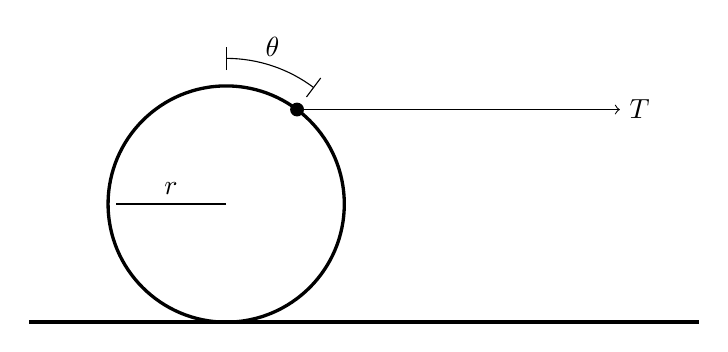
\begin{tikzpicture}[dot/.style = {circle, fill, minimum size=#1, inner sep=0pt, outer sep=0pt}]
\draw[very thick] (0,0) circle (1.5);
\draw (0,0) -- node[above]{$r$} (-1.4,0);
\node at (0.9, 1.2) [dot=5]{};
\draw[->] (0.9, 1.2) -- (5, 1.2) node[right] {$T$};
\draw[very thick] (-2.5, -1.5) -- (6, -1.5);
\draw (0, 1.7) -- (0, 2);
\draw (0, 1.85) arc (90 : 53 : 1.85) node[midway, above]{$\theta$};
\draw (1.02, 1.36) -- (1.2, 1.6);
\end{tikzpicture}
\end{center}
\end{problem}